\usetikzlibrary{shapes.geometric, arrows}

% Style for process block.
\tikzstyle{process} = [rectangle, text width=2cm, minimum width=2cm, minimum height=0.5cm,text centered, draw=black,
fill=orange!30]

% Style for terminal block.
\tikzstyle{terminal} = [rectangle, text width=2cm, minimum width=2cm, minimum height=0.5cm,text centered,
draw=black, fill=red!30]

% Style for decision block.
\tikzstyle{decision} = [diamond, text width=1.5cm, minimum width=2.2cm, minimum height=1.8cm,text centered, draw=black,
fill=green!30, inner sep=-12pt]

% Style for line.
\tikzstyle{line} = [draw, -latex']

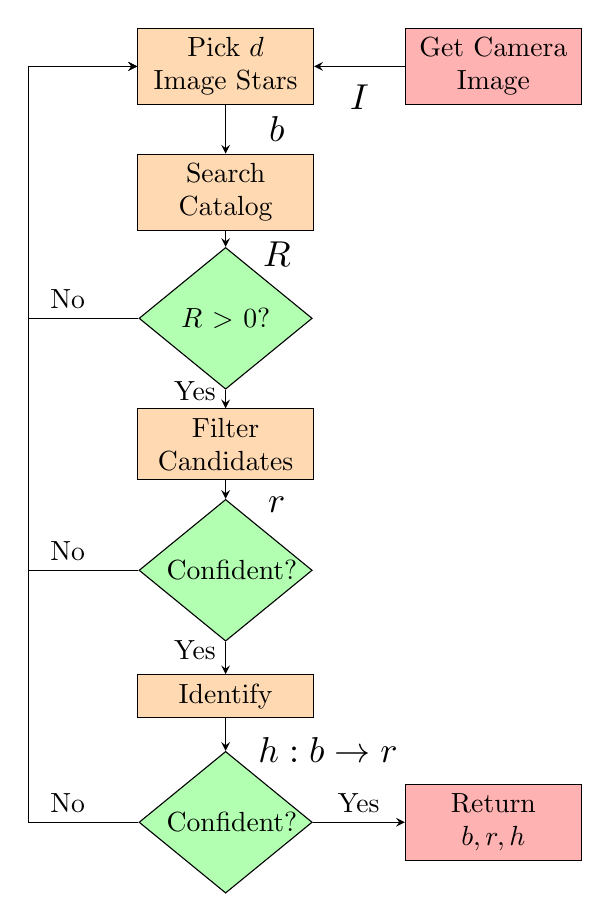
\begin{tikzpicture}[node distance=1.2cm]
    \node[scale=1](getImage)[terminal]{Get Camera Image};
    \node[scale=1](pickQueryStars) [process, left of=getImage, xshift = -2.2cm] {Pick $d$ Image Stars};
    \node[scale=1](searchCatalog)[process, below of=pickQueryStars, yshift=-0.4cm] {Search Catalog};
    \node[scale=1](confidentInCatalog)[decision, below of=searchCatalog, yshift=-0.4cm] {$\lvert R \rvert > 0$?};
    \node[scale=1](filterCandidates)[process, below of=confidentInCatalog, yshift=-0.4cm] {Filter Candidates};
    \node[scale=1](confidentAfterFilter)[decision, below of=filterCandidates, yshift=-0.4cm] {Confident?};
    \node[scale=1](findMap)[process, below of=confidentAfterFilter, yshift=-0.4cm]{Identify};
    \node[scale=1](confidentInMap)[decision, below of=findMap, yshift=-0.4cm] {Confident?};
    \node[scale=1](returnMap)[terminal, right of=confidentInMap, xshift = 2.2cm] {Return $b, r, h$};

    \draw[->,>=stealth](getImage) -- node[scale=1.3, yshift=-0.3cm]{$I$}(pickQueryStars);
    \draw[->,>=stealth] (pickQueryStars) -- node[scale=1.3, xshift=0.5cm]{$b$}(searchCatalog);
    \draw[->, >=stealth] (searchCatalog) -- node[scale=1.3, xshift=0.5cm, yshift=-0.15cm]{$R$}(confidentInCatalog);
    \draw[->, >=stealth] (confidentInCatalog) -- node[anchor=east, yshift=0.1cm]{Yes}(filterCandidates);
    \draw[->, >=stealth] (filterCandidates) --
    node[scale=1.3, xshift=0.5cm, yshift=-0.15cm]{$r$}(confidentAfterFilter);
    \draw[->, >=stealth] (confidentAfterFilter) -- node[anchor=east, yshift=0.1cm]{Yes} (findMap);
    \draw[->, >=stealth] (findMap) --
    node[scale=1.3, xshift=1cm, yshift=-0.15cm]{$h: b \rightarrow r$} (confidentInMap);
    \draw[->, >=stealth] (confidentInMap) -- node[xshift=0cm, yshift=0.25cm]{Yes} (returnMap);

    \draw[->, >=stealth] (confidentInCatalog.west) -- ++(-1.4cm, 0cm) node[anchor=south, xshift=0.5cm]{No}
    |- (pickQueryStars.west);
    \draw[->, >=stealth] (confidentAfterFilter.west) -- ++(-1.4cm, 0cm) node[anchor=south, xshift=0.5cm]{No}
    |- (pickQueryStars.west);
    \draw[->, >=stealth] (confidentInMap.west) -- ++(-1.4cm, 0cm) node[anchor=south, xshift=0.5cm]{No}
    |- (pickQueryStars.west);
\end{tikzpicture}